\chapter{Implementation}\label{ch:implementation}
This design is hierarchical. The top layer is an AES128 block in 
CBC-mode. It takes an input TS-packet, selects data from it which it 
scrambles and outputs the data in the form of a TS-packet once 
again.

The scrambler (Figure \ref{block:scrambler}) consists of two entities. 
An entity which is called the CBC-entity, which deals with the 
scrambling of the received data. The other entity is a data-manager. 
The manager deals with reading data from the interface towards the 
rest of the FPGA as well as sending data-bits to the CBC-entity at the 
correct time. It also tells the CBC-entity how to handle the data, 
since different tasks are to be done depending on if the data is the 
first data packet sent or not.

\begin{figure}[h!]
  \centering
  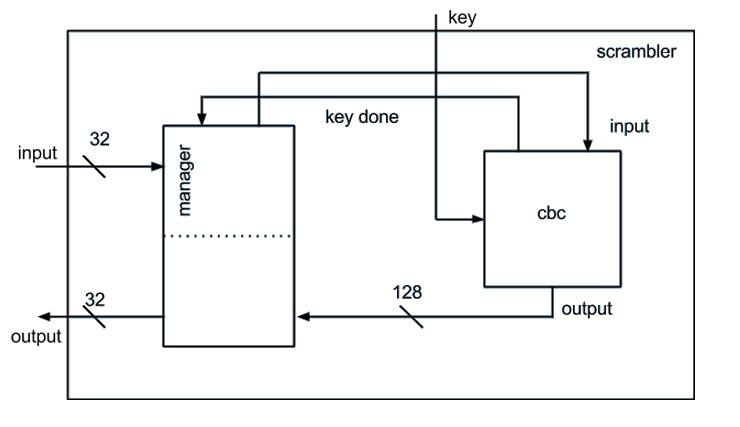
\includegraphics[width=0.75\textwidth]{scrambler}
  \caption{Scrambler-block.}
  \label{block:scrambler}
\end{figure}

\section{Manager entity}
The manager (Figure \ref{block:manager}) consists of a FIFO (First in, 
First out), an FSM (Final State Machine) and a couple of registers. 
The FIFO is needed since the data sent to the scrambler from the FPGA 
is sent in bursts. The FIFO therefore writes the data bursts into a m
emory, from which it later reads, processes and sends the data to the 
CBC-entity. The data written to the FIFO is written in packets of 32 
bits, but are read 8 bits at the time. The manager looks through the 
data packets to see if there is an adaptation field or not, since that 
changes the way that the data is handled. The payload is written to 
the first set of registers as the data is found, and then sent to the 
next set of registers. This is done to allow the manager to deal with 
two sets of data in parallell. However, only one packet is scrambled 
at any given time. When the packet is ready to be sent, a flag is set 
and the data is sent to the CBC-entity. The output of the registers 
is the input of the CBC-entity, which can be seen in figure 
\ref{block:scrambler}.

\begin{figure}[h!]
  \centering
  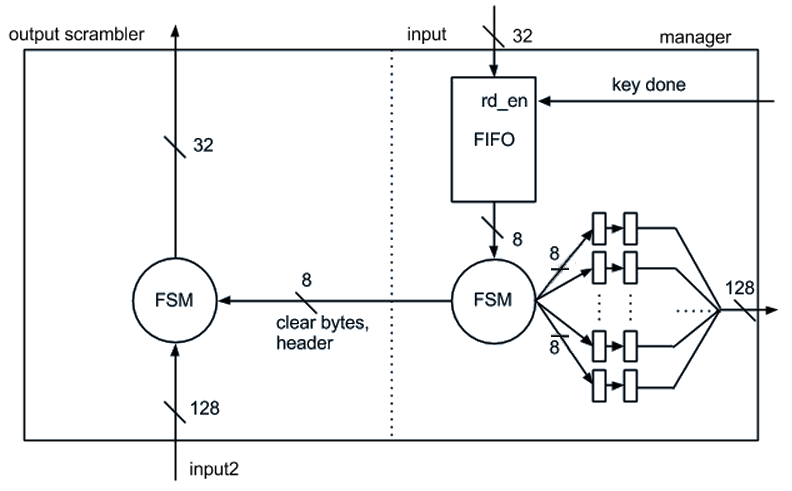
\includegraphics[width=0.75\textwidth]{manager}
  \caption{Manager-block.}
  \label{block:manager}
\end{figure}

\section{CBC entity}
The CBC-entity (Figure \ref{block:cbc}) consists of three small 
entities. An XOR, a multiplexer and a cipher-entity. The multiplexer 
is needed since the first plaintext should be sent to the XOR together 
with an IV. For the rest of the plaintexts contained within the same 
TS packet, the output ciphertext should be used instead of the IV. 
There is only going to be one AES128 cipher in the CBC-entity in 
order to save hardware. It will be run in sequence instead of in 
parallell, even though it might reduce the maximal speed of the 
circuit. CBC is explained in section \ref{sec:cbc}.

\begin{figure}[h!]
  \centering
  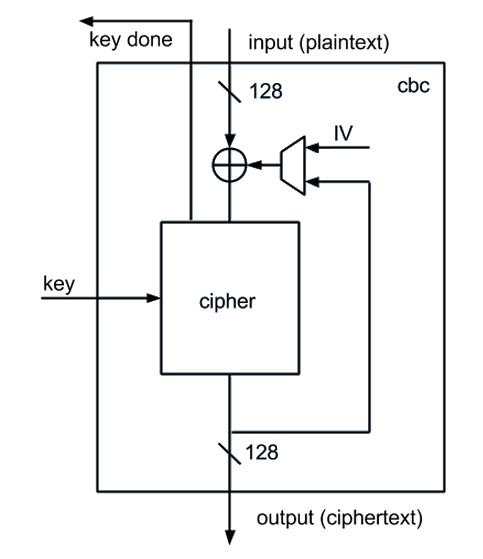
\includegraphics[width=0.75\textwidth]{cbc}
  \caption{CBC-block.}
  \label{block:cbc}
\end{figure}

\section{Cipher entity}
The AES128 cipher-entity (Figure \ref{block:cipher}) consists of 4 
components. The data2state entity, which transforms the array into a 
matrix of data. A keyexpansion entity, which takes an input of a key, 
and generates an extended key as an output. An entity, which was 
named rounds, that deals with the encryption of the 16 byte data 
blocks. And finally a state2data entity, which transforms the data-
matrix into an array once again. The cipher entity itself keeps track 
of timing mainly between the keyexpansion and the round entity. It 
uses an FSM to make sure that the round entity is provided with the 
correct roundkey at the right time, and data is output when 
it is scrambled. What can not be seen in figure \ref{block:cipher} is 
that the keyexpansion entity also sends an enable signal, that tells 
the cipher entity that the expanded key is complete.

\begin{figure}[h!]
  \centering
  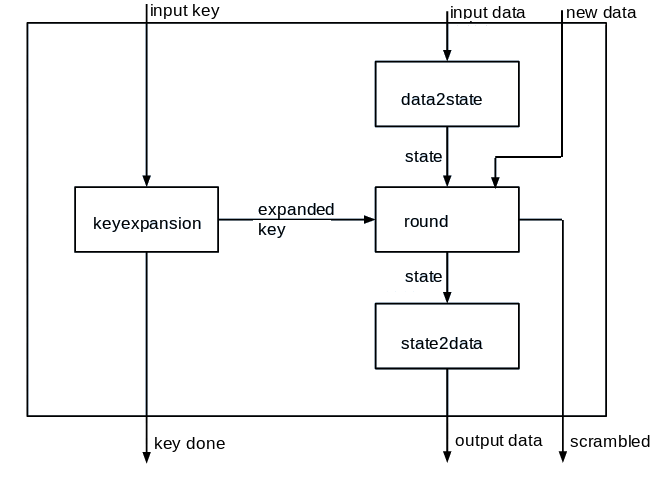
\includegraphics[width=0.75\textwidth]{cipherblock}
  \caption{Cipher-block.}
  \label{block:cipher}
\end{figure}

\section{Keyexpansion entity} \label{sec:Expansion}
The keyexpansion-entity (Figure \ref{block:keyexpansion}) is divided 
into three keyblock entities. The first keyblock entity decides what 
four bytes of the expanded key are to be expanded. The first time, the 
bytes are selected from the provided key, but after the first key has 
been expanded, the data bits are chosen from the newly expanded key. 
The second keyblock entity (Figure \ref{block:keyblock2}) contains the 
keycore, which is only performed on every fourth set of four bytes, 
and a demux entity. The third keyblock entity performs an XOR between 
either the first or second keyblock depending on if the keycore was 
supposed to be run and the key. It also increments the internal 
counter, which is used as an index when accessing and generating the 4 
byte blocks of data.

The FSM seen in figure \ref{block:keyexpansion} keeps track of when 
the key generation is done, and produces a lock signal at that time. 
The lock signal is used by keyblock3 to produce the done signal, that 
is passed to other entities. 
The FSM also keeps track of when a new key is received, and forces a 
reset of keyblock2 and keyblock3, since they are not entirely 
combinatorial. The internal reset signal, reset\_i, forces a reset of 
keyblock2 and keyblock3. 

\begin{figure}
  \centering
  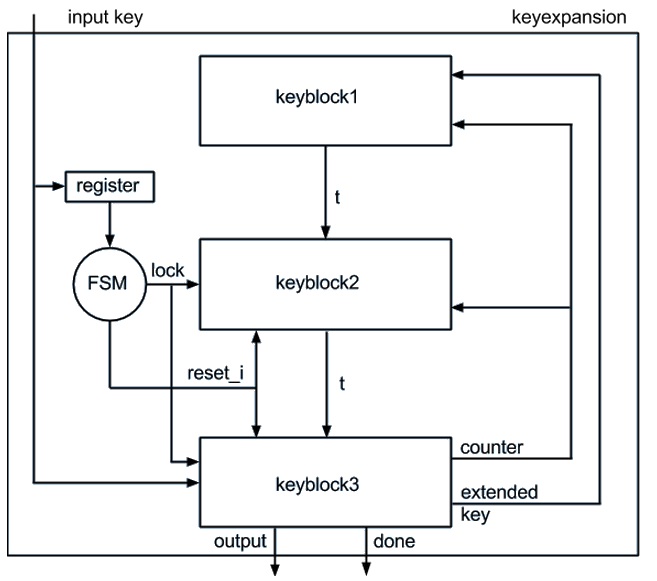
\includegraphics[width=0.75\textwidth]{keyexpansion2}
  \caption{Keyexpansion-block.}
  \label{block:keyexpansion}
\end{figure}

\begin{figure}
  \centering
  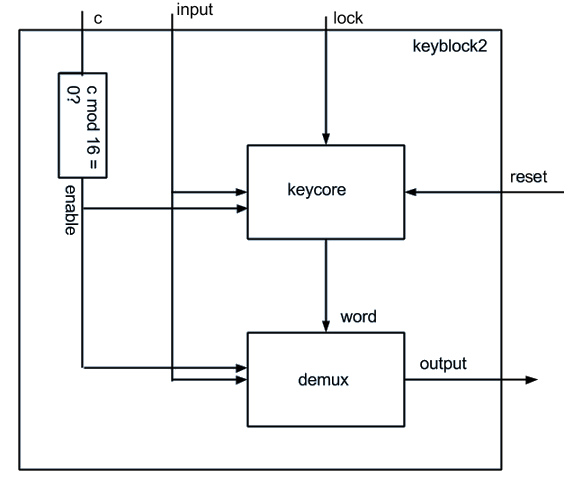
\includegraphics[width=0.75\textwidth]{keyblock2}
  \caption{Keyblock2-block.}
  \label{block:keyblock2}
\end{figure}

\subsection{Keycore entity}
The keycore entity consists of four entities. Rotword, Sbox, Rcon and 
a counter. The counter is used to get the correct output from the Rcon 
entity, and the index is only used in the keycore, and is thus best 
suited to be placed inside the keycore entity. Rotword rotates the 
bytes of the input one step to the left through a simple left shift. 
The Sbox replaces the input bytes according to the Rijndael Sbox, 
through a LUT. The Rcon entity both collects the correct rcon value 
from a precalculated vector, as well as inputs it into an xor together 
with the input.

\section{Round entity}
The round-entity (Figure \ref{block:round}) consists of four entities, 
which are called Subbytes, shiftrows, mixcolumns and addroundkey. 
Addroundkey is a special XOR, which changes input depending on what 
round is being processed. Subbytes is an Rijndael Sbox which takes an 
input 16-byte state, substitutes it and outputs another 16-byte state. 
Shiftrows shifts the rows of the second, third and fourth row of 
the state. Last, but not least, is the mixcolumns entity. It consists 
of 16 mulblock entities. The input state of mixcolumns is split into 
columns, and each column is sent to a mulblock entity, which 
multiplies the inputs with 1, 2 or 3, then performs a bitwise XOR on 
them and outputs the result of the XOR. The function of the mixcolumns 
block is a complex matrix multiplication.

\begin{figure}[h!]
  \centering
  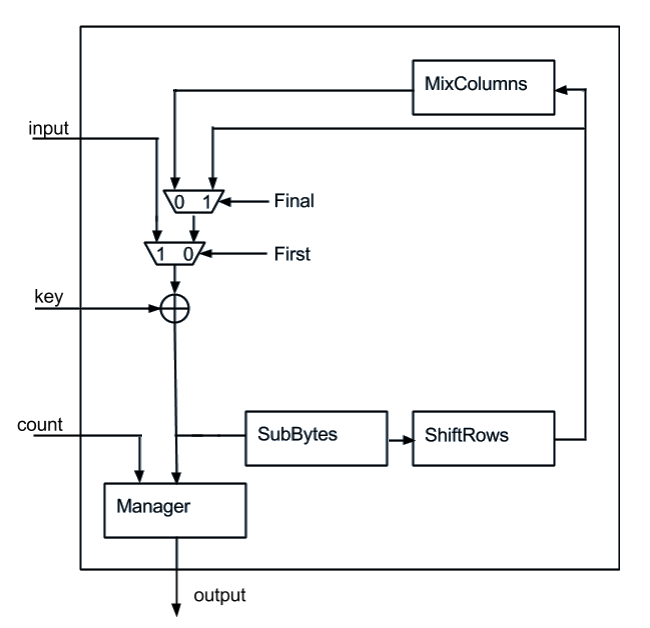
\includegraphics[width=0.7\textwidth]{round}
  \caption{Round-block.}
  \label{block:round}
\end{figure}

\subsection{Addroundkey entity}
Addroundkey is an entity which takes different inputs depending on 
what round is currently being dealt with. On the first round, 
Addroundkey takes the input to the round entity. On the last round, it 
takes the output from the ShiftRows entity. The input to addroundkey 
is the output from MixColumns the rest of the time.

\subsection{The mulblock entity}
The mulblock entity is the multiplication used by the MixColumns 
entity. It consists of one mul3 entity and one mul2 entity, which 
performs a special kind of hardware multiplication of three, and two, 
on the input. It also takes two inputs which it does not process, 
those are the values multiplied by one. The four results are then 
XOR:ed with eachother, and returned to the mixcolumns entity. The 
result is then input into the correct index in the matrix.

Mul3 means multiplication with 3, and mul2 means multiplication with 
2. A multiplication with 2 is a left-shift, followed by an XOR with 
the fix value 0x1B if the shifted value exceeds 0xFF. A multiplication 
with 3 is the same as a multiplication with 2, followed by an XOR with 
the input value. The choice of using an XOR instead of additions, and 
the XOR with 0x1B are explained in section \ref{sec:MixColumns}.
